\section{Materials and methods} 

\subsection{Programming languages and general tools}

The RNAscape webserver is a single-page web application. The backend (Figure 2A, B) is implemented in Python 3.9.18, and Django (22) is used to communicate with the backend. The frontend is (Figure 2C) designed in React v18.2.0 framework and implemented in Hypertext Markup Language (HTML)/Cascading Style Sheets (CSS)/JavaScript.

\subsection{The RNAscape algorithm}

Upon upload, the structure file is sent via Hypertext Transfer Protocol Secure (HTTPS) to the RNAscape webserver where backend processing occurs. If a user selects a PDB ID (21), its corresponding first biological assembly is downloaded by the backend (Figure 2A, B) for processing.

Pre-processing (Figure 3A). The DSSR program (v1.7.8) (20) is run on the structure file to detect helices and base pairs, and assign base-pairing annotations.

Helical regions (Figure 3B). The positioning of helices, as well as non-helical regions, involves multiple considerations. The 3D coordinates of each nucleotide are represented by the centroid of atoms belonging to it (i.e. for the nucleotide,
). The set of all nucleotide centroids is a combination of two subsets (i.e. (helical regions) and (non-helical regions)). Helical regions receive the highest priority and are placed in a way that reflects their spatial orientation while remaining visually intuitive. To do so, first, we run principal component analysis (PCA) exclusively on the helical segments () and project the points onto the plane determined by the first two components. In this process, the  sized matrix is converted to a matrix (which we can denote as ), which preserves the maximum spatial variance possible in two dimensions (23). Next, we convert into a more visually intuitive ‘ladder’ representation, which first involves estimating a ladder axis in the projection plane for each helix. An initial estimate is made by connecting the centroid of the first and last base pairs of a helical region using a line segment. consists of multiple helical regions (i.e. ). If the midpoint of a base-pair is
, the ladder axis for is the vector
rooted at the point

.

However, for bent helices, this estimate may be imprecise. To account for this case, we measure the distance
 between the centroid of the helical projection and the midpoint of the estimated ladder axis (i.e.
. If this distance is greater than 10 Å, we re-estimate the ladder axis as a combination of two line segments: one connecting the first and central base-pair centroids and another between the central and last base-pair centroids. In theory, this process can be recursively performed. In practice, however, we observe that doing so once suffices. Next, if two helical projections are within a certain distance threshold (i.e.
Å) and have similar orientations (i.e.
), we merge them and recompute the ladder axis as described above. Next, we uniformly distribute the base pairs in the ‘ladder’ formation along each ladder axis. Finally, for cases where the projection of a helix is skewed, resulting in an overly cramped ladder representation, we lengthen the ladder to reduce visual clutter. The final mapping for nucleotide points in helical regions can be denoted as Non-helical regions (Figure 3C). Loops are either preferentially bulged out in a radial curve or interpolated linearly based on a spatial density threshold (see implementation in Data Availability), depending on the chosen setting. We choose bulging by default to reduce graph overlap and crowding. For bulging out, the structure mapping algorithm computes potential layouts and performs greedy optimization to select an optimal layout. This optimization considers the total nearest-neighbor count (within 10 Å) of all members of a loop, and the orientation with the lowest number of neighbors is selected. Let us assume that the loop is connected to two nucleotides which are part of a helical region, mapped to positions
. Two possible circular layouts are computed for the loop based on
and
: bulging out in perpendicular directions
(layout ) and
(layout ), where
denotes the unit vector which is perpendicular relative to the mapping plane. In each case, the center of the layout remains at the point (
. The radius of the circular arc is either 
, if
 \AA or
 \AA, where

is the number of points in the loop. Points are uniformly distributed on the circular arc. One of the two loop orientations is selected based on minimizing the neighbor count in helical segments as follows:

Hanging single stranded regions are linearly interpolated based on its connecting mapped helix. Additional adjustments are made for certain edge cases, such as, when a linearly interpolated non-helix nucleotide exactly overlaps with another nucleotide (see implementation in Data Availability). Structures containing no helices (generally rare) are mapped solely using a PCA.

Visualization (Figure 3C). The RNAscape backend utilizes the Matplotlib (24) and NetworkX (25) packages to plot visualizations. As input, the plotting algorithm requires the mapped points, base-pairing annotations, and user-selected visual settings for a structure. As output, it generates an image that is temporarily stored (up to 48 h) on the webserver and tied to a specific user session. Structure files are not stored. The image is served to the frontend via a Django (22) server, where it can be interacted with by the user. A user can also regenerate a plot with different visual settings. In this case, we reuse the mapping output and rerun the visualization script, resulting in a faster response time than the complete computation.
\begin{center}
    \begin{figure}
    \makebox[\textwidth]{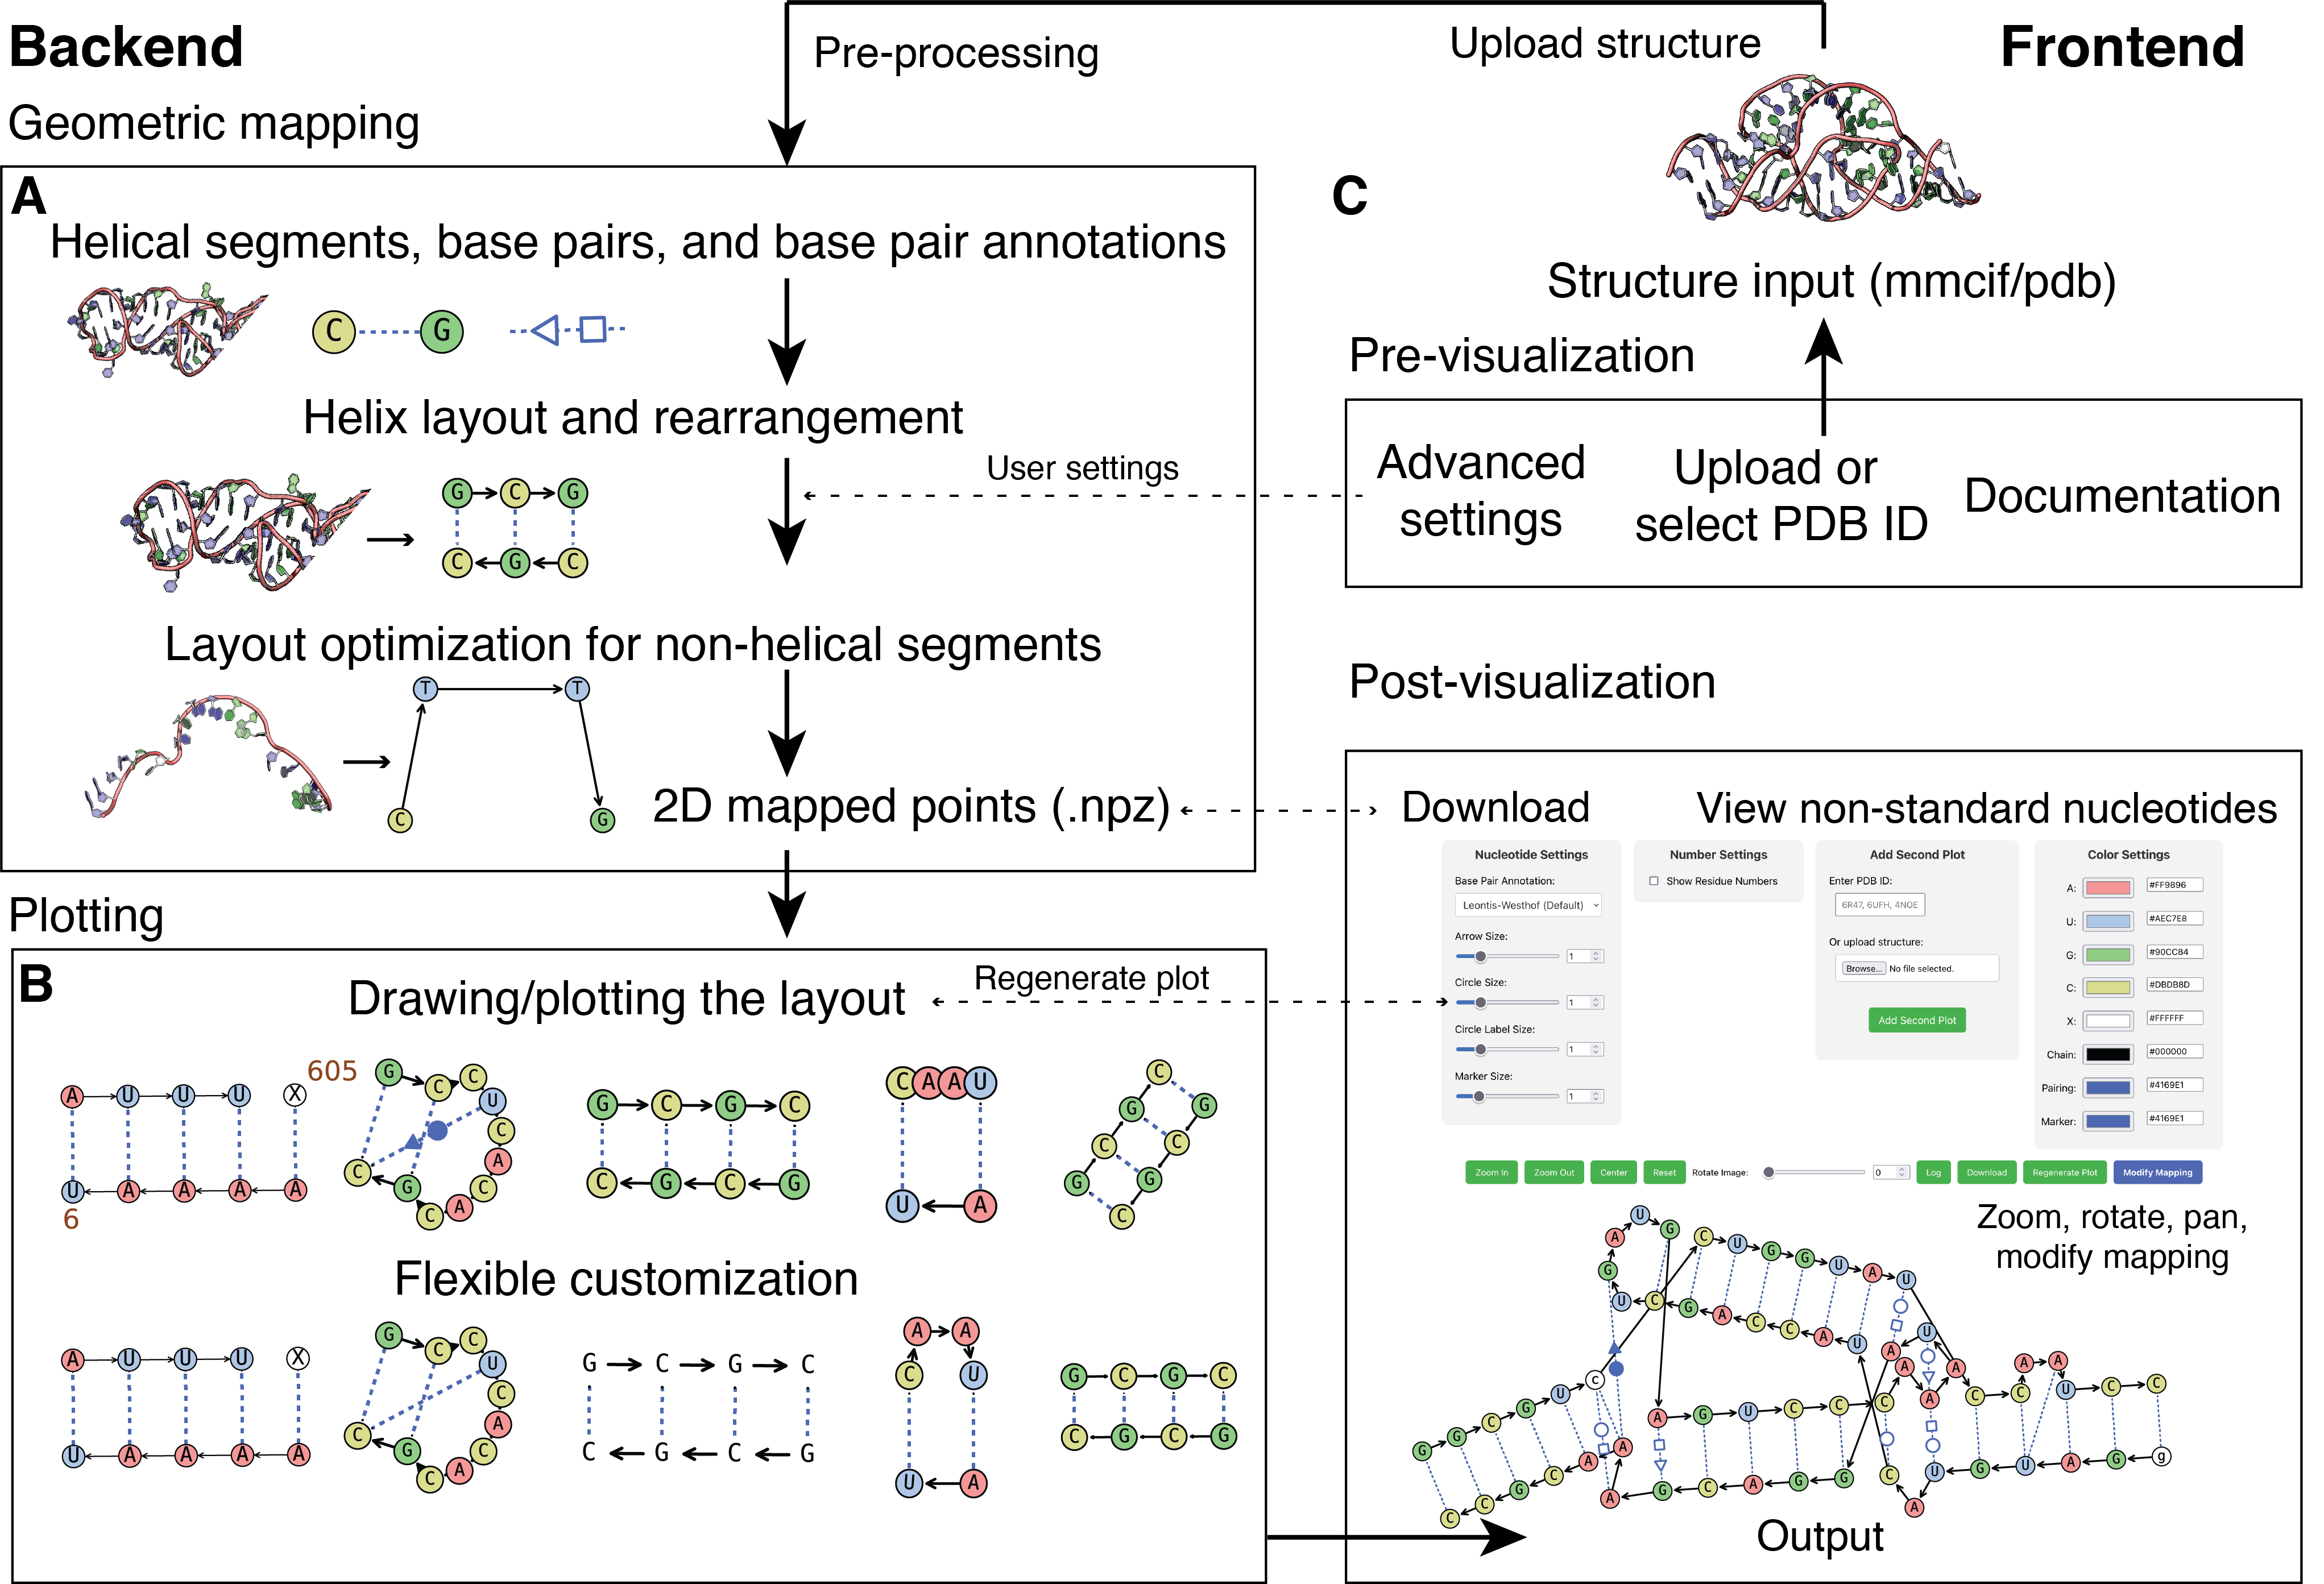
\includegraphics[width=0.8\paperwidth]{./rnascape\_figs/figure2.png}}
 % archetecture.png: 1149x508 px, 72dpi, 40.53x17.92 cm, bb=0 0 1149 508
        \caption[Computational cost of training RVAgene]{\textbf{Training RVAgene is reasonably scalable on CPU and even more so using hardware acceleration through GPU.} ({\bf A}) Time cost of training RVAgene for 100 epochs for datasets with varying number of genes and time points on CPU and GPU. ({\bf B}) Maximum memory utilized during training of the model on CPU an GPU for the cases in (A), inset plot: comparison of max memory used compared to DPGP for varying number of genes.}
  \label{fig:rnascape2}
\end{figure}
\end{center}